\section{SunDog Interior}

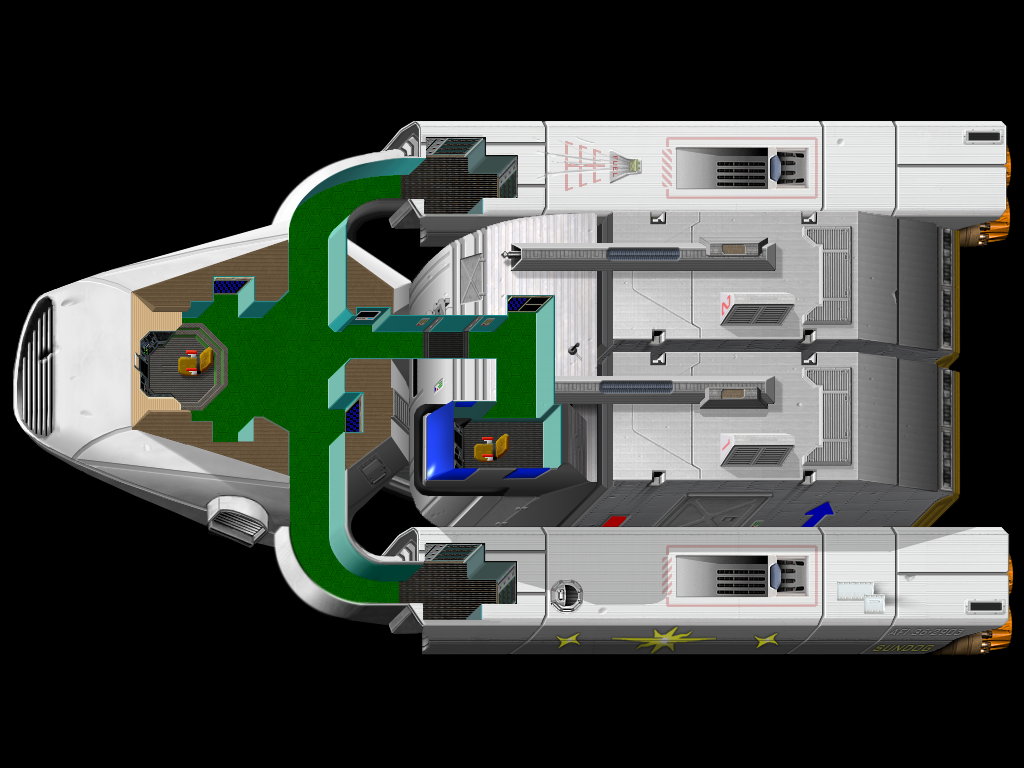
\includegraphics[scale=0.35]{images/sundog-interior-with-pod.png}



TODO:
\begin{itemize}
\item add sundog interior image without the pod
\end{itemize}

\subsection{Collision Detection}


\includegraphics[scale=0.35]{images/sundog-interior-with-pod-collidemap.png}

\subsection{Cockpit}

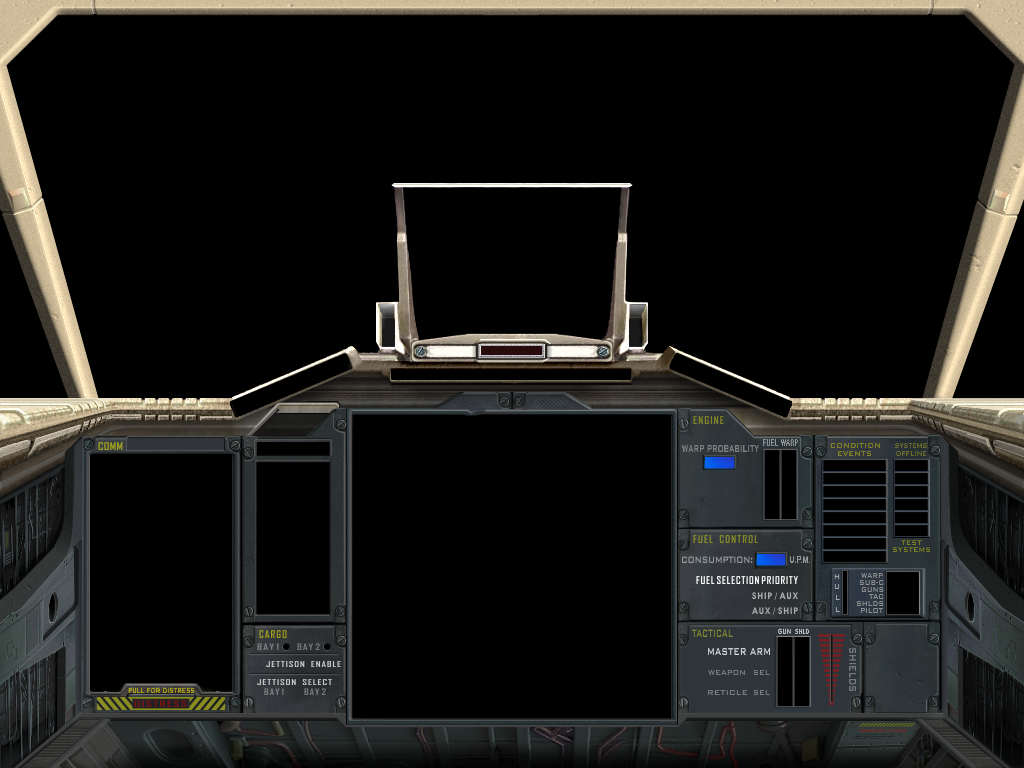
\includegraphics[scale=0.35]{images/cockpit.png}

The cockpit of the SunDog is the command center for the entire ship.  At
first the cockpit, like that of an airplane, can look like a fairly daunting
place, however, the controls are grossly simplified and should be fairly
easy to figure out.

\subsubsection{Comm}
The Comm system is used for ship-to-ship communications, and possibly, to play music on "radio stations" broadcast from planets that are within range of the Sundog.  

The comm control panel has five channels, one per button. The buttons are located in the indented strip at the top of the panel.

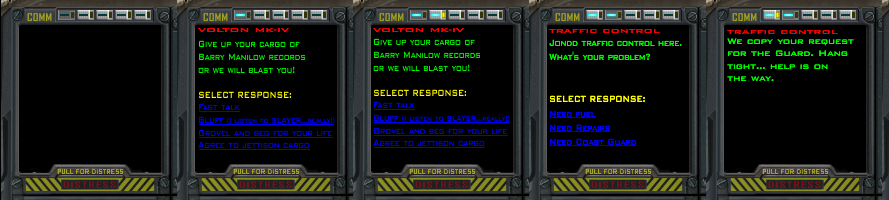
\includegraphics{images/beta COMM storyboard.png}

The comm is inactive until it receives a signal. The user can hit any of the five buttons at any time, depressing the button as is shown in comm screen #1 (far left) but nothing will show on the screen if there is no signal. (alternatively, we can have a short message like "Channel 1 - No uplink" display on the comm screen if the player pushes buttons without a signal.)

When a signal is received, it is funneled into the first unused channel - in the storyboard's case, it is the first button. When the signal comes, it lights up the button with a blue line, to show this is an active channel. An alert sound should accompany the initiation of the signal. The blue bar on the button will light up regardless of whether the channel button is currently depressed or not. (see screen #2 in the storyboard).

The message displays in the screen, with the source at the top, followed by the source's message, then by the options (like hyperlinks) for the user to select. The NPC ship replies or updates the information due to the player's non-response, and the player is given new options to respond with. Such time-out for non-response should be 30 seconds. If the player does not click one of the options within 30 seconds (regardless of whether the channel screen is visible or not) the NPC will send another message or terminate the conversation and begin shooting. (re: original game)

If during the course of the first radio conversation a second one is initiated or received, the next available comm channel button will light up blue. Moreover, it will also have a blinking yellow light, that will blink twice a second.  (See screen #3 in the storyboard). The yellow light indicates that there is an unread message on that screen.

Pushing the second channel button will switch the screen to that conversation. (See screen #4). The blinking yellow light turns out, as you now have displayed the new message. Note both channels, including the first, are lit blue, as they both have active conversations.

If during the course of the second conversation a message is received in the first conversation, the yellow light will begin to blink, indicating the new message. (see screen #5). It will continue to blink until the player switches back to that conversation.

Once a conversation is concluded, a text message should indicate this (i.e. "Uplink terminated") at the bottom of the screen under the text of the last message, and the blue light will turn off. When the user leaves the screen for another, the text (containing the NPC's last message) on the screen will be lost, and a blank screen will result if the player returns to that screen.

If a conversation terminates while the player is viewing another screen, the yellow light will blink (just as if it received a new message) and when the player changes to that channel they will see the last message and the text alert indicating the conversation is over.

The DISTRESS bar will activate if the player clicks it, and it will open a conversation with traffic control. Once clicked, the bar should remain down and lit up. After traffic control answers and then concludes the conversation (either with the player requesting help or a time-out where the player never requests anything), the distress bar should automatically spring back into place. The timeout should be 30 seconds, where if the TC answers and the player doesn't choose an option in 30 seconds, the TC will terminate the conversation.

Color scheme for text:
Red = source name and system alerts (i.e. "lost uplink", "message terminated", etc)
Green = NPC message
Yellow = Player Prompt
Blue = Player's response


MUSIC: 
For the music radio broadcast, it will work just like an incoming conversation described above, with the exception that the yellow light will never flash as it is assumed the radio broadcast is constant, regardless of a song change, etc. When the player nears a planet and is within radio range, they a channel button will light up. The comm screen will then act as a browser that will let the player switch tunes, review information, etc. This spec will be drawn up later on  (I don't expect us to worry about radio stations for a while - we have bigger fish to fry first). When the player leaves the range of the station, it will terminate and the screen will go blank.


\begin{tabular}{ | l | l | l | }
\hline
Indicator or Button & Active & Inactive \\
\hline
Distress & 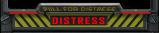
\includegraphics[scale=0.5]{images/distress_on.png} & 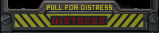
\includegraphics[scale=0.5]{images/distress_off.png} \\
\hline
\end{tabular}

Open Items:
\begin{itemize}
\item What's the response time for distress calls?  Is it different
depending on what system the ship is in (presumably some random value
which interacts with the lawlessness value)?
\item What happens when the distress call is answered?  Is a ship dispatched or
the police just call and have a conversation?  Can we show multiple
conversations on the Comm display?
the cursor up similar to the sliders?
\end{itemize}

\subsubsection{Tactical}
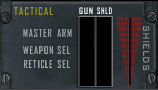
\includegraphics[scale=0.7]{images/tactical.png}

The tactical panel controls the weapons and shields systems of the SunDog.
Arming the tactical controls can be done by toggling either the "Master Arm"
button, or the "Nav/Tac" button just below the HUD.  Tactical mode can
only be entered when the SunDog is in space.

In tactical mode, the ship will yaw or pitch along with the mouse.  If
the mouse moves up, the nose of the ship will pitch down, and conversely
if the mouse moves down, the nose of the ship will pitch up.  If the
mouse is moved to the left or right, it will yaw the SunDog in either
of those directions.  The further the mouse is moved, the more the ship
will pitch or yaw.  The ship will continue to move in the same direction until
the reverse action is done (there is no friction in space!).  If the
ship is pitching upward, the mouse must be moved upward to pitch the nose
down.

The "Weapons Sel" button toggles between the ships cannon and its laser, 
which is displayed on the HUD.

When the "Reticle Sel" button is pressed the reticle on the HUD will
illuminate and stay lit for 3 seconds.  If the button is pressed again
before the reticle disappears, it will cycle to the next reticle
in the sequence.  The time that the reticle stays illuminated will
be reset to 3 seconds.

The "Gun" status indicator shows the charge of the currently selected
weapon system.  A "peak" mark will be displayed at the highest amount
the guns can charge to.  The guns status indicator will normally be in
green, however if concentrators are used the value can go past 100\%.
In this case, values above 100\% will be shown as a secondary bar in
red which overlaps the primary bar.

The "SHLD" status indicator shows the current charge of the shields and
the SHIELDS slider bar can be moved to turn on a dynamic amount of
shield power.  A "peak" mark will be displayed at the highest amount
the shields can charge to, which the shields will not charge past
even if the slider is set higher.

Art Assets:

\begin{tabular}{ | l | l | l | l | }
\hline
Indicator or Button & Active & Inactive & Misc\\
\hline
Master Arm & 
\includegraphics{images/button_danger_on.png} & 
\includegraphics{images/button_danger_off.png} & \\
Weapon Sel & 
\includegraphics{images/button_on.png} & 
\includegraphics{images/button_off.png} & \\
Reticle Sel & 
\includegraphics{images/button_on.png} & 
\includegraphics{images/button_off.png} & \\
Shields & & & 
\includegraphics{images/slider.png} \\
Gun Gauge & (255, 0, 0, 255) & & \\
Shield Gauge & (255, 0, 255, 255) & & \\
\hline
\end{tabular}

Open Items:
\begin{itemize}
\item We need to include a table of reticles that the user can cycle through.
\item How do we show the charge in the GUN indicator if the user is
using concentrators and the charge can be more than 100%?  Presumably
even if one gun row is offline the system can charge to 100% if concentrators
are being used on the other 3 rows.
\item If the shields can only work at a reduced efficiency, do they still
take the same amount of fuel to run as they would if they were 100\%?
\item The buttons are somewhat small, so do we want it to toggle them
when a user clicks on the writing as well as the button?
\end{itemize}

\subsubsection{Cargo}

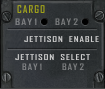
\includegraphics[scale=0.7]{images/cargo.png}

Sometimes during ship to ship fighting it becomes necessary to jettison cargo.
The "BAY 1" and "BAY 2" status lights are illuminated green (0, 255, 0, 255)
whenever cargo is present in its respective bay.  To eject cargo, the
"Jettison Enable" button must be toggled to the on position, which will
illuminate the "Jettison Select" buttons for whichever bay currently
has cargo.

After pushing a "Jettison Select" button, the cargo bay light will no longer
be illuminated and the jettison select button will become inactive.  The
indicator light should fade from green to black in 1\slash 4 of a second.

Art Assets:

\begin{tabular}{ | l | l | l | p{3.5cm} | }
\hline
Indicator or Button & Active & Inactive & Notes \\
\hline
Enable Button & 
\includegraphics{images/button_red_on.png} & 
\includegraphics{images/button_red_off.png} & \\
Jettison Select & 
\includegraphics{images/button_danger_on.png} & 
\includegraphics{images/button_danger_off.png} & \\
Bay Lights & (0, 255, 0, 255) & & The indicator should fade in or out whenever
cargo is ejected or picked up (usually by the tractor beam) \\ 
\hline
\end{tabular}

Open Items:
\begin{itemize}
\item Do we want the status light to fade out or just go 
\end{itemize}

\subsubsection{Heads Up Display}

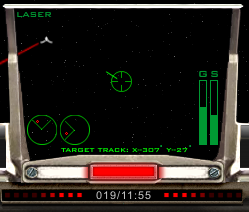
\includegraphics[scale=0.7]{images/hud.png}

The heads up display is the main tactical viewport of the Sun Dog.  When
tactical mode is activated, the HUD will illuminate its center reticle
and the tracking circles for fighting enemy ships.  In addition, tracking
information is display in the lower portion of the view port and the
weapon selected will be displayed in the upper left hand corner.


Open Issues:
\begin{itemize}
\item The Guns\slash Shields indicators are redundant to the ones on
the dash board.  Do we need to show them in two places?
\item Does the red alert light stay on or does it flash?  Should this be
drawn programatically or should we use an image?
\item Do we need to show the Z coordinate along with X and Y of attacking
ships?
\item Do we want to use the fancy warp effects that we had for the 2D
game?
\item The reticle depicted has an extra line which appears to point toward
where the attacking ship is.  Do we want a reticle that can do this?
\end{itemize}

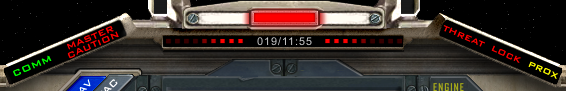
\includegraphics[scale=0.7]{images/lower-hud.png}

Below the HUD is the red alert indicator which should activate when the
SunDog is under attack.

A chronometer with the current game time is displayed underneath the red
alert indicator and a pulsing strip surrounds it which signals that the ships
Sub-C engines are currently activated.

Open Issues:
\begin{itemize}
\item How does the COMM indicator work?
\item When does the MASTER CAUTION indicator come on?  When tactical mode
is activated?
\item Is it the THREAT LOCK indicator or the THREAT and LOCK indicators,
and when are they activated?  Is this when the enemy locks onto the SunDog
or when the SunDog is using something like the autoslew part?
\item What does the PROX indicator do?
\end{itemize}

\subsubsection{Primary Flight Display}

Open Issues:
\begin{itemize}
\item Need to mock up the various screens for how this is going to work.
\end{itemize}

\subsubsection{Computer}

Open Issues:
\begin{itemize}
\item There should be some way of changing ship settings such as yaw vs.
roll.
\item There needs to be an option to tractor beam in cargo after
destroying an enemy vessel.
\item We need to mock up the various situations for what menu items
will show up in the computer.  Also, does the tactical mode make sense?
\item Was the Nav\slash Tac button above the computer supposed to change modes
of the computer or was it supposed to automatically put the SunDog into
tactical mode?
\end{itemize}

\subsubsection{IFF}

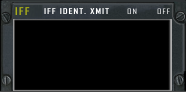
\includegraphics[scale=0.70]{images/iff.png}

When the SunDog comes across another vessel or object in space, the ship's
onboard IFF system will display information about the object.  

Art Assets:

\begin{tabular}{ | l | l | }
\hline
Ship or Visual & Image \\
\hline
Angolith MK-V & \\
Annihilator & \\
Cryn MK-90 & \\
Cryn MK-110 & \\
Cryn MK-140 & \\
Death Angel MK-2 & \\
Debris Field & \\
Jammed Signal & \\
Kolum 8820 & \\
Life Pod & \\
Gorathi M5 & 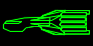
\includegraphics[scale=0.75]{images/ship_gorathi_m5.png} \\
Phantom UL & 
\includegraphics[scale=0.75]{images/ship_Phantom_UL.png} \\
Probe & \\
Rathain M1 & \\
Rathain M5 & \\
Rynroth-VOR & \\
Shath Class 3 & \\
Skryth MK-IV & 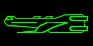
\includegraphics[scale=0.75]{images/ship_skryth_mk-iv.png} \\
Skryth MK-VII & \\
Sorth CF-50 & 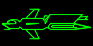
\includegraphics[scale=0.75]{images/ship_sorth_cf-50.png} \\
Space Station & \\
Space Station & \\
Unknown Enlie & \\
Valshur 85 & \\
Valshur 130 & \\
Vestar Class II & 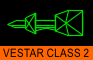
\includegraphics[scale=0.75]{images/ship_vestar_class_2.png} \\
Volton MK-IV & 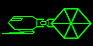
\includegraphics[scale=0.75]{images/ship_Voton_MK_IV.png} \\
Volton MK-X & 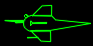
\includegraphics[scale=0.75]{images/ship_Voton_MK_X.png} \\
VW 69 & 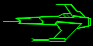
\includegraphics[scale=0.75]{images/ship_VW-69.png} \\
Z1 - Vector & \\
\hline
\end{tabular}

Open Issues:
\begin{itemize}
\item IFF ident buttons are to be removed.
\item Fill in the rest of the wireframes.
\item Are certain ships more likely in certain places with less lawlessness?
\item What are the different capabilities of each of the ships?
\item It would be nice to do a rotating wireframe of each ship.
\item We need to have corresponding 3D models to each of the ship outlines.
\end{itemize}

\subsubsection{Engine}
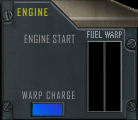
\includegraphics[scale=0.70]{images/engine.png}

Open Issues:
\begin{itemize}
\item Remove the engine start button.
\item The warp charge entry needs to be changed to the successful warp
probability meter.
\end{itemize}

\subsubsection{Fuel Control}
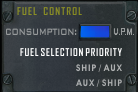
\includegraphics[scale=0.70]{images/fuelcontrol.png}

Fuel control shows the current fuel drain on the ship, and allows the player
to decide whether to draw fuel from an auxillary fuel pod, or from the
ship's fuel tanks.  Fuel drain is calculated at in "Units Per Minute" for
each of the ships systems.

The "Ship\slash Aux" button in the fuel control panel will default to
being illuminated.  If there is an auxillary fuel pod onboard, pressing
"Ship\slash Aux" or "Aux\slash Ship" will cause whichever button was
pressed to be illuminated and the other button to be inactive.  Otherwise
"Ship\slash Aux" will always be active.  Fuel will drain from whichever
supply is selected until it runs out, at which point it will start to drain
from the other supply.  

When fuel runs out, all systems except the Comm will be inoperative and
the "Systems Offline" and "Low Fuel" indicators will become illuminated.

Fuel Consumption Rates:

\begin{tabular}{ | l | l | }
\hline
Ship System & Rate \\
Cannon\slash Laser & 10\slash minute \\
Guns Idle & 2\slash minute \\
Shields & 20\slash minute while charging \\
Shields Idle & 2\slash minute \\
Sub-C & 35\slash minute \\
Warp & 45\slash minute while charging \\
Warp Idle & 2\slash minute \\
Cloaker & 80\slash minute \\
Decloaker & 50\slash minute \\
Idle Consumption & 1\slash minute \\
\hline
\end{tabular}

Open Issues:
\begin{itemize}
\item If the "AUX\slash SHIP" button is pushed when there is no auxillary
fuel pod, is there still a sound emitted?
\item How do we want to handle refueling?  Will the systems automatically
all come back online?
\item Should there be fuel drain for systems which are not working at
peak efficiency?  This could be a huge gameplay issue since it could make
combat too difficult if parts are popping in the middle of combat which
causes fuel drain to increase.
\end{itemize}

\subsubsection{EPU System}

The Emergency Power Unit is a system of last resort for powering the
SunDog to quickly get to a particular place, at the cost of running
out of all remaining fuel.

Open Issues:
\begin{itemize}
\item Remove the EPU from the cockpit.
\end{itemize}

\subsubsection{Indicators}
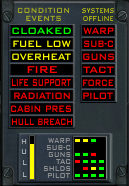
\includegraphics[scale=0.70]{images/indicators.png}

The system indicators are broken down in to several catagories, namely
condition events, offline systems, hull status and system status.

Each row of every system will be displayed as a green, yellow or red
indicator in the system status window depending on their status.  An
offline row (one with a broken or missing part) will not be illuminated.
If all rows are offline, the functionality of that system is considered
offline and a red indicator light will illuminate in the "Systems Offline"
indicator panel.

The "FUEL LOW" indicator is illuminated when there are only 200 units
of fuel left total (from both the main tank and the aux tank).

The "HULL" inidcator shows the current state of the hull up to 100%.
Between 95-100\%, the indicator will be green (0, 255, 0, 255),
yellow between 30-94\%, otherwise red.  If the hull gets to 0\%, the
space ship is destroyed. 

%\begin{inparaenum}[\itshape a\upshape\)]
%\item condition events;
%\item offline systems;
%\item hull status; and
%\item system status
%\end{inparaenum}

Open Issues:
\begin{itemize}
\item When does an "OVERHEAT" event happen?  From the ships guns?  After
how many times would that happen from firing?
\item When would life support be compromised?  How long until the player dies?
Do we even need a concept of life support?
\item What does it mean when there is a hull breach?  Can the hull be breached
only when the hull meter is at zero?
\item What does the cabin pressure light do?  Is this redundant to 
the hull breach indicator?
\item What does a radiation event do?  Is that when there is a problem with
a ships system or is it when the SunDog flies too close to the sun?  Do
we need this option?
\item In the mockup it says "FORCE" instead of "SHLDS" for the system
offline indicator.  Do we care about this (maybe we leave it as a cute
quirk)?
\item We 
\item How does hull indicator work?  Should it be different colours depending
on how damaged the hull is?
\end{itemize}

\subsection{System Bays}
The SunDog contains a number of system bays which control various aspects of
the ships' functionality.  Each of the bays require certain parts which are
necessary for the smooth operation of each individual system.  From time to
time, various parts will wear out or will become inoperative during certain
high stress times such as ship-to-ship combat.  If enough parts of a particular
system have been damaged, the system will go offline and will have to be
repaired.  This can create some potentially difficult situations if the
SunDog is engaged in combat and systems like shields or guns become
inoperative.  It is highly beneficial to have an extra supply of parts in
case things go wrong!

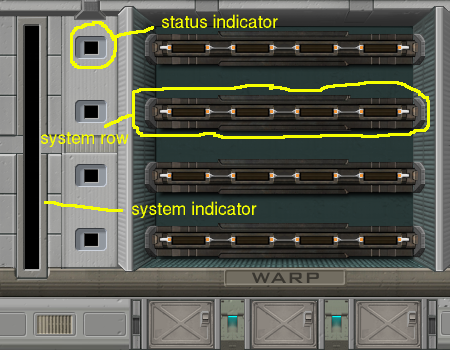
\includegraphics[scale=0.70]{images/interior-warp.png}

Each system bay contains four rows of parts, and each row can take a
combination of parts which is unique to that system bay.  Each row of
parts contributes 1/4 of the capability of a given system and all parts
in a given row need to be functioning for the row to work.

System parts are modular and can be plugged in to any slot that accepts the
same part.  Most slots can also take a "shunt", which is a universal part
which will allow the row to function, but in a reduced capacity.  Shunts
also have an uncanny ability to fail when they are most needed, so the use
of shunts should probably be avoided unless necessary.

A status row next to each system row indicates the current performance
of that row.  A green light indicates that the row is operating at
100\% capacity.  If a shunt is used for any part in the row, the row will
operate at 76\% capacity and the inidicator light will be yellow.  If
more than one shunt is used in the row, the indicator light will be red
and the row output will be 48\% for two shunts and 24\% for three shunts.

\subsubsection{Pilotage}

\begin{tabular}{ | p{2.5cm} | p{2.5cm} | p{2.5cm} | p{2.5cm} | }
\hline
Slot 1 & Slot 2 & Slot 3 & Slot 4 \\ \hline
Control Node & J-Junc Module & Scanner & J-Junc Module \\
& Shunt & Shunt & Shunt \\
& & Ground Scanner & \\
\hline
\end{tabular}

Open Issues:
\begin{itemize}
\item What functionality does pilotage give the ship?
\end{itemize}

\subsubsection{Guns}

\begin{tabular}{ | p{2.5cm} | p{2.5cm} | p{2.5cm} | p{2.5cm} | }
\hline
Slot 1 & Slot 2 & Slot 3 & Slot 4 \\ \hline
Control Node & Cryo Fuse & Photon Bridge & Plasma Tube \\
& Shunt & Shunt & Shunt \\
& Cloaker & & \\
\hline
\end{tabular}

The gun bay controls the operation of the cannon and laser systems aboard
the SunDog.  Without working guns the SunDog it is impossible to strike
back at attacking ships during ship-to-ship combat.

Open Issues:
\begin{itemize}
\item To what degree will the efficiency of the guns systems affect
combat effectiveness?
\item Is the laser weaker in the case that the system is not running
at peak efficiency?  Presumably no but it will take longer to charge --
the charge can determine the damage to the other ship.
\item Is the cannon weaker?  Does it take more fuel to fire?
\end{itemize}

\subsubsection{Shields}

\begin{tabular}{ | p{2.5cm} | p{2.5cm} | p{2.5cm} | p{2.5cm} | }
\hline
Slot 1 & Slot 2 & Slot 3 & Slot 4 \\ \hline
Control Node & Cryo Fuse & Flux Modulator & Flux Modulator \\
& Shunt & Shunt & Shunt \\
& Cloaker & & \\
\hline
\end{tabular}

The shields system controls the ships shields which prevent damage to
the hull and system parts when the SunDog is under attack.  Without
properly working shields the SunDog will become damaged very quickly
if it takes a direct hit from enemy cannon or laser fire.

Open Issues:
\begin{itemize}
\item How does the shield efficiency affect the operation of the shields?
Presumably the efficiency determines the percentage to what the shields can
be raised to:  ie. 100\% efficiency and the shields can be raised 100\%.
With shields at 25\%, they could only be raised 25\%.
\item How does the shield efficiency determine the rate of damage?
\end{itemize}

\subsubsection{Sub-C}

\begin{tabular}{ | p{2.5cm} | p{2.5cm} | p{2.5cm} | p{2.5cm} | }
\hline
Slot 1 & Slot 2 & Slot 3 & Slot 4 \\ \hline
Control Node & Flux Modulator & ST Distorter & Cryo Fuse\\
& Shunt & Shunt & Shunt \\
\hline
\end{tabular}

Open Issues:
\begin{itemize}
\item Is the sub-light speed directly proportional to the efficiency
of the engines?  ie. if the system is at 75\% capacity, will it take
133\% as much time to arrive as it would if the engines were working at
100\%?
\end{itemize}

\subsubsection{Tactical}

\begin{tabular}{ | p{2.5cm} | p{2.5cm} | p{2.5cm} | p{2.5cm} | }
\hline
Slot 1 & Slot 2 & Slot 3 & Slot 4 \\ \hline
Control Node & Scanner & J-Junc Module & Photon Bridge \\
& Shunt & Shunt & Shunt \\
\hline
\end{tabular}

Open Issues:
\begin{itemize}
\item Presumably tactical would adversely affect the way the thrusters
work when maneuvering during combat.  Is there any other affect?
\end{itemize}

\subsubsection{Warp}

\begin{tabular}{ | p{2.5cm} | p{2.5cm} | p{2.5cm} | p{2.5cm} | }
\hline
Slot 1 & Slot 2 & Slot 3 & Slot 4 \\ \hline
Control Node & Flux Modulator & Photon Bridge & ST Distorter \\
& Shunt & Shunt & Shunt \\
\hline
\end{tabular}

Open Issues:
\begin{itemize}
\item Do the warp engines only determine the distance that the SunDog
can jump?  ie. if you have only one system row working, can the SunDog
only jump 1/4 the distance?
\end{itemize}

